%\documentclass[a0,landscape]{a0poster}
\documentclass[a0]{a0poster}
\pagestyle{empty}
\setcounter{secnumdepth}{0}
\usepackage[absolute]{textpos}
\usepackage{graphicx}
\usepackage{times}
\usepackage{color}
\usepackage{url}
\usepackage{amsmath}
\usepackage{amsfonts}
\usepackage{amssymb}
\usepackage{natbib}
\usepackage{caption}
\usepackage{tikz}
\usepackage{array}
\usetikzlibrary{arrows.meta}

\definecolor{DarkBlue}{rgb}{0.4,0.4,1}
\definecolor{Red}{rgb}{0.9,0.0,0.1}
\definecolor{Black}{rgb}{0.0,0.0,0.0}
\definecolor{Green}{rgb}{0.0,0.9,0.1}

\DeclareMathOperator{\KL}{KL}
\DeclareMathOperator{\Tr}{Tr}

% Custom color titles
\let\Textsize\Large
\def\Head#1{\begin{center}\noindent{\LARGE\bf\color{Black}#1}\end{center}\bigskip}
\def\LHead#1{\noindent{\Large\color{Black} #1}\smallskip}
\def\Subhead#1{\begin{center}\noindent{\Large\color{Black}#1}\end{center}\smallskip}
\def\Title#1{\noindent{\Huge\bf\color{Black} #1}}


% ----------------------------------------------------------------------------
% TITLE SECTION
% ----------------------------------------------------------------------------
\begin{document}
\vspace{0.5cm}
\hspace{2cm}
% UdeM Logo
\begin{minipage}{0.15\textwidth}
    \flushleft
    
\includegraphics[width=\columnwidth]{figures/udem}
\end{minipage}
\hfill
% Title and Authors
\begin{minipage}{0.6\textwidth}
      \centering
      \baselineskip=3\baselineskip
      \Title{\begin{center}Deep Active Localization\end{center}}
      \vspace{-1cm}
      \LHead{\begin{center}
      Sai Krishna*$^\dagger$ \hspace{2cm} Keehong* \hspace{2cm} Dhaivat Bhatt $^\dagger$ \hspace{2cm} Vincent Mai $^\dagger$
      \hspace{2cm} Krishna Murthy $^\dagger$
      \hspace{2cm} Liam Paull $^\dagger$
      \end{center}}
      \vspace{-1.8cm}
      \LHead{\begin{center}
        {\it\rmfamily $^\dagger$Montreal Institute for Learning Algorithms }
      \end{center}}
      \vspace{-2cm}
\end{minipage}
\hfill
% MILA Logo
\begin{minipage}{0.15\textwidth}
    \flushright
    
\includegraphics[height=.4\columnwidth]{figures/mila}
\end{minipage}
\hspace{2cm}
\vspace{2cm}
\\
% Black line
\begin{minipage}{1.\textwidth}
    {\color{Black}{\vrule depth 0pt height 0.3cm width \columnwidth}}
    \vspace{0.5cm}
\end{minipage}
\hfill
% ----------------------------------------------------------------------------
% FIRST COLUMN
% ----------------------------------------------------------------------------
\begin{minipage}[t]{0.32\textwidth}
    % Introduction 
    \Head{Overview}
    \vspace{1cm}
    \begin{minipage}{1.0\columnwidth}
        \Large
{\color{blue}{\textbf{Problem Statement:}}}Assuming that the agent is placed at some point in the map, find the sequence of control inputs, $u_{1:T}$ that allow it to maximally disambiguate its pose within the map.



{\color{blue}{\textbf{Approach:}}}
We jointly train likelihood model and policy model on simulator using domain randomization which facilitates efficient transfer of the learned models to real world.
        \vspace{1cm}
    \end{minipage}

    % Background
    \Head{Background}
    \vspace{1cm}
    \begin{minipage}{1.0\columnwidth}
    \Large
    A \emph{disentangled representation} has single latent dimensions sensitive to single generative factors, while being relatively invariant to changes in other factors.
    \end{minipage}\\[1.5cm]
    \begin{minipage}{1.0\columnwidth}
    	\Large{\color{blue}{\textbf{Variational Autoencoder (VAE)}}}
        \begin{itemize}
        	\item Suppose we have a latent variable model $p(\mathbf{x}, \mathbf{z})$ with a \emph{complex likelihood model} $p_{\theta}(\mathbf{x}\ |\ \mathbf{z})$ (e.g. a Normal distribution, with mean parametrized by a deep neural network with parameters $\theta$).
            \item We use \emph{amortized variational inference} to approximate the true posterior $p(\mathbf{z}\ |\ \mathbf{x})$ (intractable) with a distribution $q_{\phi}(\mathbf{z}\mid \mathbf{x})$ (e.g. a Normal distribution with diagonal covariance, parametrized by a deep neural network with parameters $\phi$).
            \item The model $p_{\theta}(\mathbf{x}\mid \mathbf{z})$ and posterior approximation $q_{\phi}(\mathbf{z}\mid \mathbf{x})$ are trained jointly by maximizing the \emph{Evidence Lower Bound} (ELBO):
            \begin{equation}
            	\mathcal{L}(\theta, \phi\,;\,\mathbf{x}) = \mathbb{E}_{q_{\phi}(\mathbf{z}\mid \mathbf{x})}\left[\log p_{\theta}(\mathbf{x}\mid \mathbf{z})\right] - \KL(q_{\phi}(\mathbf{z}\mid \mathbf{x})\,\|\,p(\mathbf{z}))
            \end{equation}
        \end{itemize}
		\Large{\color{blue}{\textbf{$\beta$-VAE}}}
		\begin{itemize}
			\item In $\beta$-VAE, we introduce a single hyperparameter $\beta$ (usually $\beta \geq 1$) and replace the ELBO objective by
            \begin{equation}
            	\mathcal{L}(\theta, \phi\,;\,\mathbf{x}) = \mathbb{E}_{q_{\phi}(\mathbf{z}\mid \mathbf{x})}\left[\log p_{\theta}(\mathbf{x}\mid \mathbf{z})\right] - \beta\, \KL(q_{\phi}(\mathbf{z}\mid \mathbf{x})\,\|\,p(\mathbf{z}))
            \end{equation}
            \item Higher values of $\beta$ create a trade-off between between reconstruction quality and interpretable latent representation by increasing the importance of making the distribution $q_{\phi}(\mathbf{z}\mid \mathbf{x})$ close to an isotropic Gaussian.
		\end{itemize}
\begin{minipage}{\columnwidth}
	\vspace{1cm}
	\centering
  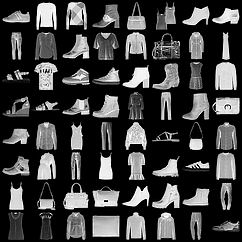
\includegraphics[width=0.32\textwidth, trim={0 5.3cm 0 0}, clip]{fashion-mnist/original.png}
  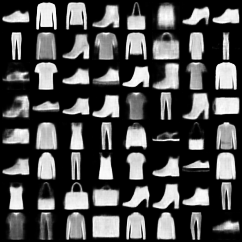
\includegraphics[width=0.32\textwidth, trim={0 5.3cm 0 0}, clip]{fashion-mnist/beta1.png}
  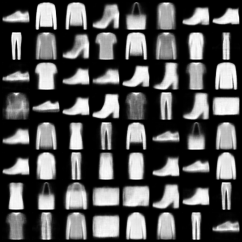
\includegraphics[width=0.32\textwidth, trim={0 5.3cm 0 0}, clip]{fashion-mnist/beta4.png}\\
  \begin{tikzpicture}[x=12.3cm]
  	\node at (0, 0) {\normalsize $\beta = 1$};
  	\node at (-1, 0) {\normalsize Original};
  	\node at (1, 0) {\normalsize $\beta = 4$};
  \end{tikzpicture}
  \vspace{1cm}
\end{minipage}
	\end{minipage}

%\vspace{2cm}
%\center{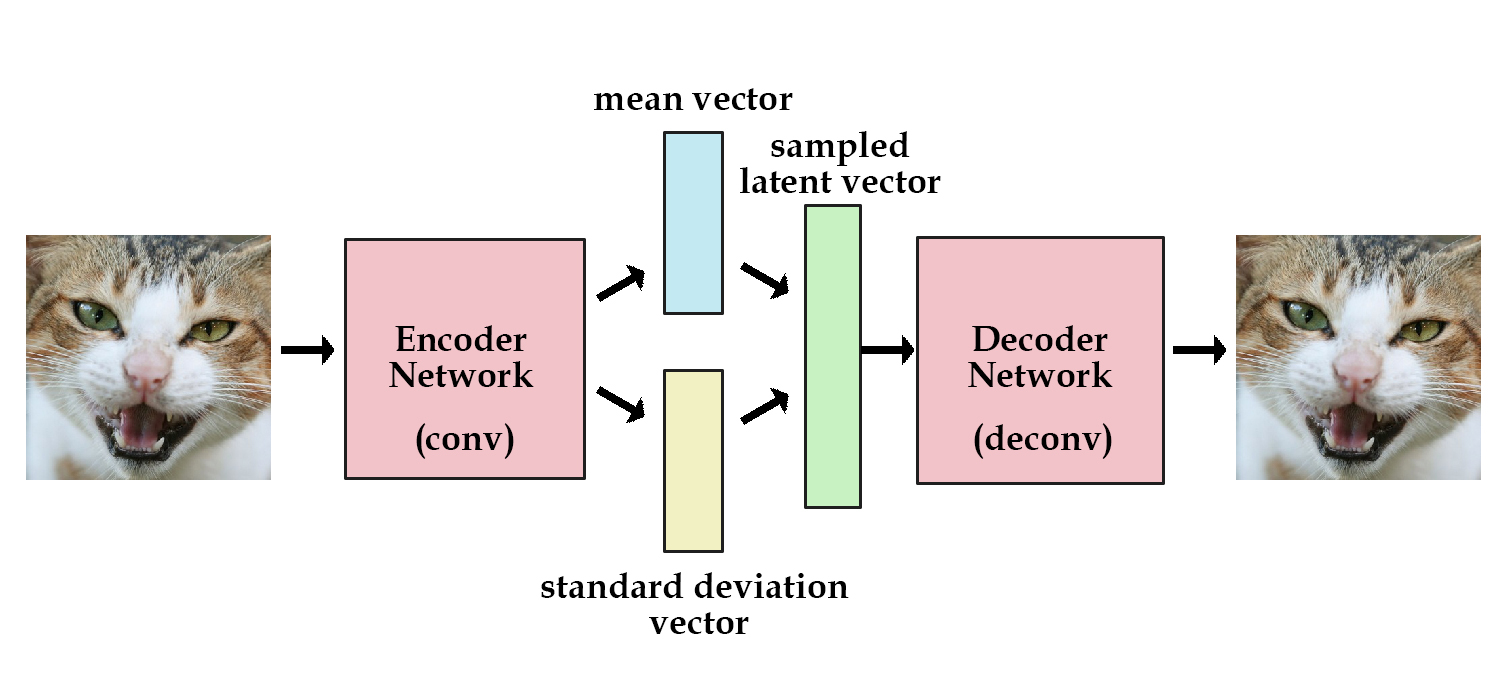
\includegraphics[width=.7\textwidth]{figures/basicvae.jpg}}
%        \vspace{2cm}
    %\end{minipage}
\Large
{\color{blue}{\textbf{Code:}}} https://github.com/montrealrobotics/dal 
    
\end{minipage}
\hfill
% ----------------------------------------------------------------------------
% SECOND COLUMN
% ----------------------------------------------------------------------------
\begin{minipage}[t]{0.32\textwidth}
    % Experiment 1
    \vspace{0cm}
    \begin{minipage}{1.0\columnwidth}
    \Large
   %{\centering
%{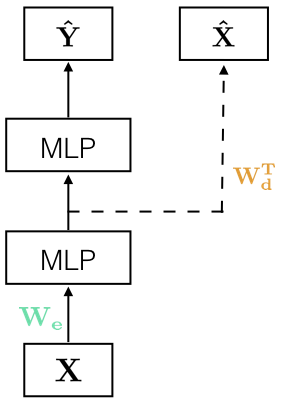
\includegraphics[width=0.35\textwidth]{figures/net_basic.png}\captionsetup{labelformat=empty}}\hfill\hspace{1cm}
%{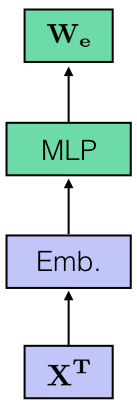
\includegraphics[width=0.18\textwidth]{figures/net1.png}}\hfill\hspace{1.5cm}
%{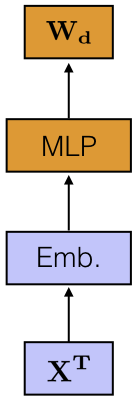
\includegraphics[width=0.18\textwidth]{figures/net2.png}}\hfill
%\vspace{1cm}\\
%\textit{Left: Basic Discriminative Network. Middle-Right: Auxiliary Networks.}}
%\vspace{1cm}\\
{\color{blue}{\textbf{Divergence}}}
\begin{itemize}
	\item {\Large While KL divergence is used in practice, the Jensen Shannon divergence and the Hellinger distance is commonly used in statistics and Wasserstein showed promising results in GANs. We bring them to the VAE domain and show comparative results.}
\end{itemize}
\begin{minipage}{\columnwidth}
	\vspace{1cm}
	\centering
  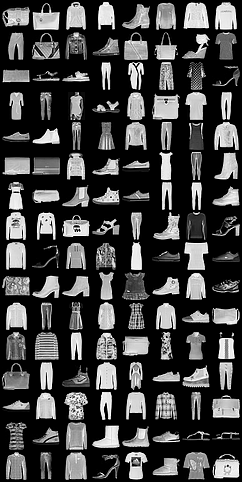
\includegraphics[width=0.19\textwidth, trim={0 13.75cm 3.15cm 0}, clip]{figures/original.png}
  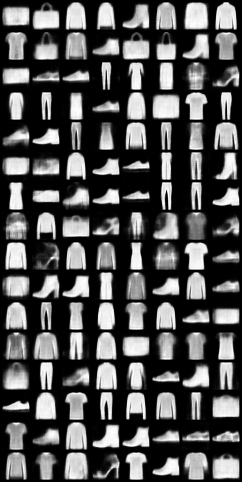
\includegraphics[width=0.19\textwidth, trim={0 13.75cm 3.15cm 0}, clip]{figures/fashion_kld_reconst_sai.png}
  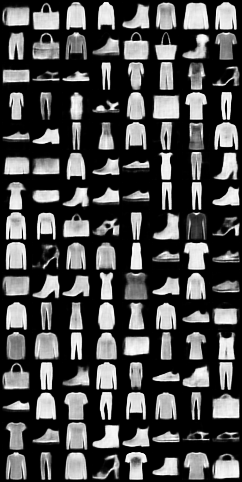
\includegraphics[width=0.19\textwidth, trim={0 13.75cm 3.15cm 0}, clip]{figures/fashion_jensen_reconst_sai.png}
  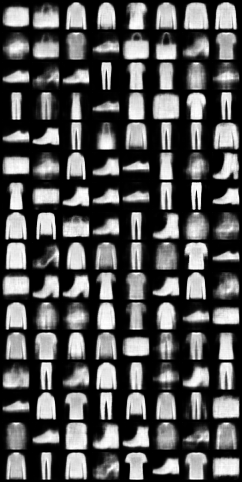
\includegraphics[width=0.19\textwidth, trim={0 13.75cm 3.15cm 0}, clip]{figures/fashion_hellinger_reconst_sai.png}
  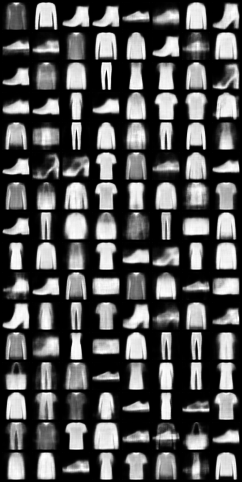
\includegraphics[width=0.19\textwidth, trim={0 13.75cm 3.15cm 0}, clip]{figures/fashion_wasserstein_reconst_sai.png}\\
  \hspace*{1.4cm}\begin{tikzpicture}[x=7.3cm]
  	\node at (0, 0) {\normalsize Jensen-Shannon\phantom{g}};
  	\node at (-2, 0) {\normalsize Original\phantom{g}};
  	\node at (-1, 0) {\normalsize Kullback- Leibler\phantom{g}};
  	\node at (1, 0) [align=center] {\normalsize Hellinger\\[-0.5em] \normalsize $\beta=10000$ };
  	\node at (2, 0) [align=center] {\normalsize   Wasserstein\phantom{g}\\[-0.5em] \normalsize$\beta=500$};
  \end{tikzpicture}
  \vspace{1cm}
\end{minipage}
% \large \begin{equation}
%             	H(P,Q)^2 = 1 - \frac{|\Sigma_{1}|^{1/4} \cdot |\Sigma_{2}|^{1/4}}{|\frac{\Sigma_{1}+\Sigma_{2}}{2}|^{1/2}} \exp\left[-\frac{1}{8} (\mu_{1}-\mu_{2})^T \left(\frac{ \Sigma_{1}+\Sigma_{2}}{2}\right)^{-1} (\mu_{1}-\mu_{2}) \right]   
%             \end{equation}
% \begin{itemize}
% 	\item {\Large Wasserstein distance}
% \end{itemize}
% 	\begin{equation}
%             	W_{2}(P,Q)^2 = \|\mu_{1}-\mu_{2}\|^2 + \Tr(\Sigma_{1} + \Sigma_{2} - 2(\Sigma_{2}^{1/2}\Sigma_{1}\Sigma_{2}^{1/2})^{1/2})
%                 \end{equation}
% \begin{itemize}
% 	\item {\Large KL div}
% \end{itemize}
% \begin{equation}
%             	KLD(P,Q) = \frac{1}{2}\left[\Tr(\Sigma_{2}^{-1}\Sigma_{1}) + (\mu_{2}-\mu_{1})^T\Sigma_{2}^{-1}(\mu_{2}-\mu_{1}) - k + \log\frac{|\Sigma_{2}|}{|\Sigma_{1}|}\right]
% \end{equation}
% \newline figure
% \vspace{1cm}

% \Large
% {\color{blue}{\textbf{Iterative:}}} Computes hidden representations $\mathbf{h_i}$, output prediction $\mathbf{\hat{y}_i}$ and reconstruction $\mathbf{\hat{x}_i}$ of one sample $\mathbf{x_i}$ as follows
% \begin{equation}
% \mathbf{h_i} = f(\mathbf{x_i}), \quad
% \mathbf{\hat{y_i}} = g(\mathbf{h_i}), \quad
% \mathbf{\hat{x_i}} = r(\mathbf{h_i}),
% \end{equation}
% where $f$, $g$ and $r$ are non-linear functions.

% The number of parameters of the first hidden layer of the architecture grows linearly with the dimensionality of . 
% \vspace{1cm}
\end{minipage}
% \begin{minipage}{1.0\columnwidth}
% 	\Large {\color{blue}\textbf{Controlled capacity increase}}
%     \begin{itemize}
%     	\item We control the encoding of the VAE's latent representation with a \emph{controlled capacity objective}
%         \begin{equation}
%         	\mathcal{L}(\theta, \phi\,;\,\mathbf{x}) = \mathbb{E}_{q_{\phi}(\mathbf{z}\mid \mathbf{x})}\left[\log p_{\theta}(\mathbf{x}\mid \mathbf{z})\right] - \gamma\, |\KL(q_{\phi}(\mathbf{z}\mid \mathbf{x})\,\|\,p(\mathbf{z})) - C|
%         \end{equation}
%         \item $C$ is gradually increasing from $0$ to a large enough to produce a good reconstruction quality.
%     \end{itemize}
% \end{minipage}\\[1cm]

\Head{Analysis}
    \vspace{1cm}
    \begin{minipage}{1.0\columnwidth}
    \begin{minipage}{1.0\columnwidth}
    \begin{minipage}[t]{0.6\textwidth}
 \Large {\color{blue}{\textbf{Disentanglement metric}}}
 \begin{itemize}
 	\item We run inference on images (dSprites dataset) generated by fixing the value of one generative factor (e.g. the scale) while randomly sampling all others.
    \item We use a linear classifier to predict this fixed factor. The accuracy of this classifier is the \emph{disentanglement metric score}.
 \end{itemize}
 \end{minipage}\hfill
 \begin{minipage}[t]{0.37\textwidth}
+ \end{minipage}
 \vspace{1cm}
 \end{minipage}
  \Large {\color{blue}{\textbf{Reproducing Kernel Hilbert Space Disentanglement Metric}}}
  \begin{itemize}
  \item Gretton et al \citep{Gretton:2005:MSD:2101372.2101382} introduce an independence criterion based on the eigenspectrum of covariance operators in Reproducing Kernel Hilbert spaces (RKHS), consisting of an empirical estimate of the Hilbert-Schmidt norm of the cross-covariance operator.
  \item We compute the empirical HSIC norm for every pair of the latent variable and report the average value below. Lower value of the metric indicates more independence
  \end{itemize}
    \vspace{0.1cm}
    \end{minipage}
%\vspace{-1.5cm}
\vspace{0.1cm} 
\Head{Results}
\vspace{0.1cm}
     {\Large \color{blue}{\textbf{RKHS dependency metric}}}\\[1cm]
     \begin{minipage}{\columnwidth}
     	\Large
        \centering
       \begin{tabular}{|>{\centering}m{10cm}|c|c|}
       	\hline
          \textbf{Model} & \textbf{Dataset} &  \textbf{RKHS dependency metric score}\\
          \hline
          VAE &  & $1.99 \times 10^{-2}$\\
          $\beta$-VAE ($\beta = 4$) & CelebA & $1.21 \times 10^{-2}$\\
          $\beta$-VAE \cite{higgins2016beta} &  &  $\mathbf{4.04\times 10^{-3}}$\\
          \hline
         VAE &  & $9.95 \times 10^{-3}$\\
          $\beta$-VAE ($\beta = 4$) & dSprites &  $8.47 \times 10^{-3}$\\
          $\beta$-VAE \cite{higgins2016beta} &  & $\mathbf{3.83 \times 10^{-4}}$\\
          \hline
      \end{tabular}
      \vspace{1cm}
\end{minipage}
\end{minipage}
%        - 0.0199564348078
%       - 0.012167895315
 %      - 0.00404160873589
\hfill
% ----------------------------------------------------------------------------
% THIRD COLUMN
% ----------------------------------------------------------------------------
\begin{minipage}[t]{0.32\textwidth}
    % Some other Stuff 
    % Conclusion
    \vspace{0cm}
    \begin{minipage}{1.0\columnwidth}
    \Large
     {\color{blue}{\textbf{Interpolation in the latent space}}}\\[1cm]
     \begin{minipage}{1.0\columnwidth}
     \centering
     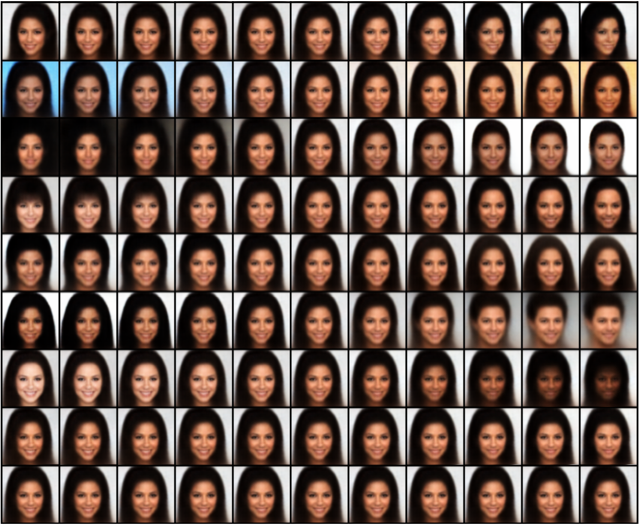
\includegraphics[width=0.6\textwidth]{celeba/disentanglement-clip.png}
     \begin{tikzpicture}[y=2.01cm, every node/.style = {anchor=west}]
     	\node at (0, 0) {\normalsize $\mathbf{z}_{5}$};
        \node at (0, -1) {\normalsize $\mathbf{z}_{6}$};
        \node at (0, -2) {\normalsize $\mathbf{z}_{8}$};
        \node at (0, -3) {\normalsize $\mathbf{z}_{9}$};
        \node at (0, -4) {\normalsize $\mathbf{z}_{13}$};
        \node at (0, -5) {\normalsize $\mathbf{z}_{19}$};
        \node at (0, -6) {\normalsize $\mathbf{z}_{25}$};
        \node at (0, -7) {\normalsize $\mathbf{z}_{28}$};
        \node at (0, -8) {\normalsize $\mathbf{z}_{\text{unused}}$};
     \end{tikzpicture}
     \end{minipage}\\[0.5cm]
     \hspace*{5.4cm}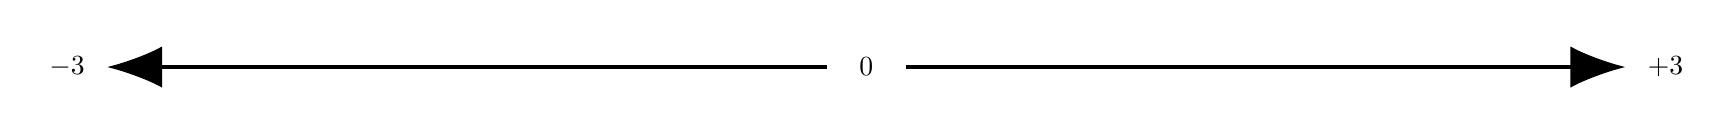
\begin{tikzpicture}[x=20.3cm]
     	\node[minimum size=1cm] (A) at (0, 0) {\normalsize $-3$};
        \node[minimum size=1cm] (B) at (1, 0) {\normalsize $+3$};
     	\draw[{Latex[length=7mm]}-{Latex[length=7mm]}, line width=1.2pt] (A) -- (B) node [midway, minimum size=1cm, fill=white] {\normalsize $0$};
     \end{tikzpicture}
    \vspace{1cm}
  \end{minipage}
  \begin{minipage}{1.0\columnwidth}
  
     {\Large \color{blue}{\textbf{Disentanglement metric}}}\\[1cm]
     \begin{minipage}{\columnwidth}
     	\Large
        \centering
       \begin{tabular}{|>{\centering}m{10cm}|c|}
       	\hline
          \textbf{Model} & \textbf{Disentanglement metric score}\\
          \hline
          PCA \cite{higgins2016beta} & $84.9\pm 0.4\%$\\
          ICA \cite{higgins2016beta} & $42.03\pm 10.6\%$\\
          \hline
          VAE & $59.9 \pm 1.5\%$\\
          $\beta$-VAE ($\beta = 4$) & $67.3 \pm 3.2\%$\\
          $\beta$-VAE \cite{higgins2016beta} & $\mathbf{99.23\pm 0.1\%}$\\
          \hline
      \end{tabular}
      \vspace{1cm}
     \end{minipage}

    \end{minipage}
    \Head{Conclusion}
    \begin{minipage}{0.99\columnwidth}
        \Large
        \begin{itemize}
        \item We implement VAE and $\beta$-VAE and run them on various datasets
        \item We compare the disentangling of  our $\beta = 1$, $\beta = 4$ and \cite{higgins2016beta} quantitatively and qualitatively.
        \item We see that we still have room for improvement by tuning $\beta$, potentially by attempting exponential annealing
        
%            \item We compared VAE to $\beta$-VAE 
%            \item We proposed various variants of $\beta$-VAE and leave it for further research to combine 2 or more of those techniques and obtain SOTA  
%            \item We showed that we are awesome and give us A+ if you want your name on our publication.
        \end{itemize}
        \vspace{0cm}
    \large
    \bibliographystyle{unsrt}
    \nocite{*}
	\bibliography{./references.bib} 
    \end{minipage}
    \vspace{1cm}
\end{minipage}
\hfill
\end{document}
